\documentclass[xcolor=dvipsnames]{beamer}
\usepackage[T1]{fontenc}
\usepackage[utf8]{inputenc}
\usepackage{float}
\usepackage{pbox} %encadrement de texte
\usepackage{graphicx} %images
\usepackage[french]{babel}
\usepackage{tikz}
\usepackage{amsmath}
\usepackage{wrapfig} %figures laterales
\usepackage{pifont}% http://ctan.org/pkg/pifont
\newcommand{\cmark}{{\color{Green}\ding{51} }}%
\newcommand{\xmark}{{\color{Red}\ding{55} }}%
\usepackage{lipsum} %génération de lipsum

\graphicspath{{./slide_img/}}%

\usetheme{Madrid}
\setbeamertemplate{navigation symbols}{}


\title[]{Théorie de la Communication et de l'Information}
\author[Benjamin B., Pierre-Loup P., Pauline R.]{Benjamin Barbesange, Pierre-Loup Pissavy, Pauline Ribeyre}
\institute{ISIMA -- ZZ1 -- Communication}
\date{10 avril 2015}


\AtBeginSection[]{%
	\begin{frame}
		\frametitle{Sommaire}
		\tableofcontents[currentsection, hideothersubsections]
	\end{frame}
}
\begin{document}
	\begin{frame}[plain] %title
		\titlepage
	\end{frame}
	\begin{frame} %summary
		\frametitle{Sommaire}
		\tableofcontents[]
	\end{frame}
  \section{Principes généraux}

\begin{frame}
	\begin{block}{Communication}
		\begin{itemize}
			\item{Entre 2 organismes}
			\item{Modification de l'action del'autre}
			\item{Transmission d'unformation}
			\item{Action indirecte}
		\end{itemize}
	\end{block}
\end{frame}

\begin{frame}
	\begin{block}{Schéma de \textbf{Laswell} (1948)}
		\begin{itemize}
			\item{Qui ?}
			\item{Dit quoi ?}
			\item{Par quel moyen}
			\item{A qui ?}
			\item{Avec quel effet ?}
		\end{itemize}
	\end{block} \pause

	\begin{block}{Schéma de \textbf{Laswell} (1948)}
		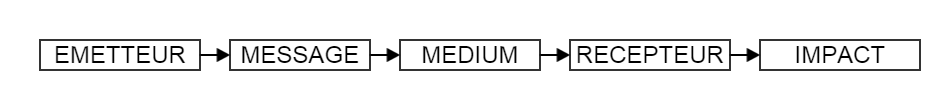
\includegraphics[width=12cm]{laswell.png}
		\begin{itemize}
			\item{Emetteur : source de l'émission}
			\item{Message : ce qui apporte l'information}
			\item{Récepteur : celui qui reçoit le message}
		\end{itemize}
	\end{block}
\end{frame}

\begin{frame}
	\begin{block}{Shannon (1949)}
		\textbf{Théorie de l'information} 
		
\includegraphics[width=12cm]{shannon.png}
		\begin{itemize}
			\item{Codage : transmission de l'information suivant un système de règles}
			\item{Décodage : lors de la réception de l'information}
			\item{Canal : voie de circulation des messages}
		\end{itemize}
	\end{block}
\end{frame}

\begin{frame}
	\begin{block}{Wiener (1949)}
		\textbf{Régulation : le feed back} 
		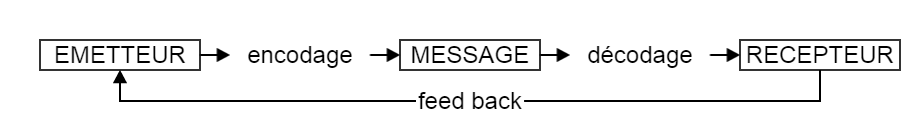
\includegraphics[width=12cm]{wiener.png}
		\begin{itemize}
			\item{Feed back : information de retour. Influe sur l'emetteur qui réajuste donc le message}
			\item{Bruits : ce qui dénature le message}
			\item{Référent : situation et contexte qui amènent à formuler le message}
		\end{itemize}
	\end{block}
\end{frame}

  %\section{Fonctions du message}

\begin{frame}
	\frametitle{Les types de messages}
	\begin{block}{Skinner (1947)}
		\begin{itemize}
			\item{Les demandes}
			\item{Les dénominations}
		\end{itemize}
	\end{block} \pause
	
	\begin{exampleblock}{Exemple}
		\begin{itemize}
			\item{"Ma poupée"}
			\item{"Donne-moi ma poupée" : demande}
			\item{"Voici ma poupée" : dénomination}
		\end{itemize}
	\end{exampleblock}
\end{frame}


\begin{frame}
	\frametitle{Les types de communication}
	\begin{block}{Zajonc (1966)}
		\begin{itemize}
			\item{Communication incidente} \pause
			\item{Communication consommatoire} \pause
			\item{Communication instrumentale}
		\end{itemize}
	\end{block}
\end{frame}


\begin{frame}
	\frametitle{Les fonctions du message}
	\begin{block}{Jakobson (1958)}
		\begin{center}
		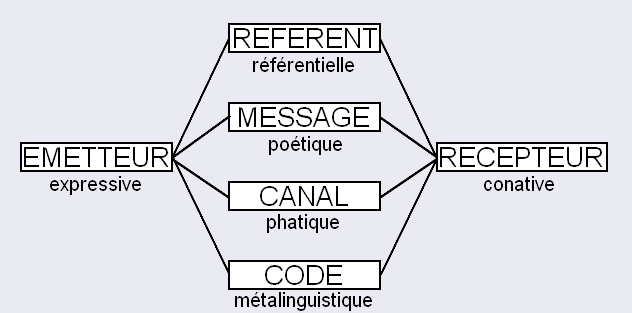
\includegraphics[height=4cm]{jakobson.png}
		\end{center}
	\end{block} \pause
	
	\begin{block}{Jakobson (1958)}
		\begin{columns}
			\begin{column}{.5\textwidth}
				\begin{itemize}
					\item{Fonction expressive} \pause
					\item{Fonction conative} \pause
					\item{Fonction référentielle} \pause
				\end{itemize}
			\end{column}
			\begin{column}{.5\textwidth}
				\begin{itemize}
					\item{Fonction phatique} \pause
					\item{Fonction métalinguistique} \pause
					\item{Fonction poétique}
				\end{itemize}
			\end{column}
		\end{columns}
	\end{block}
\end{frame}

  \section{Incertitude et information}

\begin{frame}
	\begin{block}{Quantité d'information}
		\begin{itemize}
			\item{Probabilité d'apparition d'un mot dans le message}
			\item{Probabilité élevée = peu d'information}
		\end{itemize}
	\end{block} \pause
	
	\begin{exampleblock}{Un exemple}
		\begin{itemize}
			\item{M. Dupont est Français} \pause
			\item{M. Dupont est cruciverbiste}
		\end{itemize}
	\end{exampleblock}
\end{frame}

\begin{frame}
	\begin{block}{Quantité d'information}
		Plus le message est imprévisible plus il apporte d'information
	\end{block} \pause
	
	\begin{alertblock}{Attention}
		Trop de termes imprévisibles entraînent une compréhension difficile du message
	\end{alertblock}
\end{frame}

  %\section{Coût et Redondance}

\begin{frame}
	\frametitle{Coût}
	\begin{block}{Définition}
		Durée d'utilisation d'un canal dans la transmission d'un message.
		\begin{itemize}
			\item Téléphone: Temps de communication.
		\end{itemize}
	\end{block}
	\pause
	\begin{alertblock}{Economie}
		\centering
		\begin{tikzpicture}
			\node (R) at(0,0) {Répétition importante};
			\node (M) at(6,0) {Message simplifié};
			\draw[->, thick] (R) to[bend left] (M);
			\node at(3,.75) {Contraction};
		\end{tikzpicture}
	\end{alertblock}
	\pause
	\begin{exampleblock}{Exemples}
		\begin{itemize}
			\item Métro (\emph{Métropolitain}),
			\item Périph (\emph{Boulevard Périphérique}),
			\item Labo (\emph{Laboratoire}),
			\item USA, OGM, Bio...
		\end{itemize}
	\end{exampleblock}
\end{frame}

\begin{frame}
	\frametitle{Coût}
	\begin{alertblock}{Risques}
		\centering
		\begin{tikzpicture}
			\node (P) at (0,1.5) {Phrases longues et complexes}; \pause
			\node (C) at (6,1.5) {Coût important};
			\draw[->, thick] (P)--(C); \pause
			\node (F) at (6,0) {Fatigue de l'interlocuteur};
			\draw[->, thick] (C)--(F); \pause
			\node (D) at (0,0) {Déconnexion};
			\draw[->, thick] (F)--(D); \pause
			\node[color=red] (R) at (3,-1.5) {Message non-reçu};
			\draw[->, thick] (D)--(R); \pause
		\end{tikzpicture}
	\end{alertblock}
	\begin{exampleblock}<6->{Conséquence}
		\[ \text{Diminuer le nombre de signes} \implies \text{Message plus compréhensible} \]
		$\implies$Exemple: Télégramme.
	\end{exampleblock}
\end{frame}
\begin{frame}
	\frametitle{Efficacité}
	\begin{alertblock}{Problèmes}
		\begin{itemize}
			\item Bruits parasites (environnement par exemple),
			\item Pertes d'information (discours hâché au téléphone)...
		\end{itemize}
		Equilibre nécessaire entre coût et qualité de réception.
	\end{alertblock}
	\pause
	\begin{block}{Finalement}
		\begin{itemize}
			\item Ni trop bref,
			\item Ni trop complexe.
		\end{itemize}
	\end{block}
\end{frame}
\begin{frame}
	\frametitle{Efficacité}
	\begin{exampleblock}{Origine}
		Fréquence d'utilisation des mots
		\[ \text{Trop de noms} \implies \text{Difficile} \]
	\end{exampleblock}
	\pause
	\begin{block}{Rendre le discours compréhensible}
		\emph{Degré d'intelligibilité} d'un message:
		\begin{itemize}
			\item Fréquence d'apparition,
			\item Nature des mots.
		\end{itemize} \pause
		Importance de la répartition des informations selon la \emph{prévisibilité} des termes.

		\vspace{0.2cm}
		Exemple: {\itshape"Substantifique... ?"}
	\end{block}
\end{frame}
\begin{frame}
	\frametitle{Redondance}
	\begin{block}{Objectifs}
		\begin{itemize}
			\item Assurer la qualité de la réception,
			\item Augmenter l'impact sur le récepteur,
			\item Outil de contrôle pour le récepteur.
		\end{itemize}
	\end{block}
	\pause
	\begin{exampleblock}{Définition}
		Excédent de signes pour une quantité d'information égale.
	\end{exampleblock}
	\pause
	\begin{block}{Caractéristiques}
		Emploi:
		\begin{itemize}
			\item Faible dans la communication automatique (entre machines),
			\item Indispensable dans la communication entre humains.
		\end{itemize}

		Conséquence: le \emph{coût}.
	\end{block}
\end{frame}
\begin{frame}
	\frametitle{Redondance}
	\begin{block}{Nécessité}
		Doute:
		\begin{itemize}
			\item Qualité de la réception,
			\item Système de référence,
			\item Code,
			\item Habitudes du récepteur.
		\end{itemize}

		Conditionne l'efficacité.
	\end{block}
	\pause
	\begin{exampleblock}{Redondance naturelle}
		\begin{itemize}
			\item Geste,
			\item Communication entre personnes.
		\end{itemize}
	\end{exampleblock}
\end{frame}


\end{document}
